\ZSFmanualColumnBreak
\section{Algorithmen: Sortieren}\label{sec:04-algorithmen}

\subsection{Übersicht: Sortier-Laufzeiten}\label{sec:04-übersicht-sortier-laufzeiten}
\ZSFindex[sortieren]{Sortieren}
\begin{tablebox}
\begin{ZSFtable}[\ZSFfontTableDense][\ZSFtableRowStretchRoomy]{Q{1.2} Y{0.9} Y{0.9}}
\toprule
\ZSFkeyword*{Algorithmus} & \ZSFkeyword*{Durchschnitt} & \ZSFkeyword*{Worst-Case} \\
\midrule
Bubble Sort           & $\Theta(n^2)$      & $\Theta(n^2)$ \\
Selection Sort        & $\Theta(n^2)$      & $\Theta(n^2)$ \\
Insertion Sort        & $\Theta(n^2)$ \emph{(best: $\Theta(n)$)} & $\Theta(n^2)$ \\
Merge Sort            & $\Theta(n \log n)$ & $\Theta(n \log n)$ \\
Quick Sort            & $\Theta(n \log n)$ & $\Theta(n^2)$ \\
Heap Sort             & $\Theta(n \log n)$ & $\Theta(n \log n)$ \\
Binary Insertion Sort & $\Theta(n^2)$      & $\Theta(n^2)$ \\
\bottomrule
\end{ZSFtable}
\end{tablebox}

\begin{contentbox}[Details: Vergleiche und Vertauschungen]
\begin{center}
    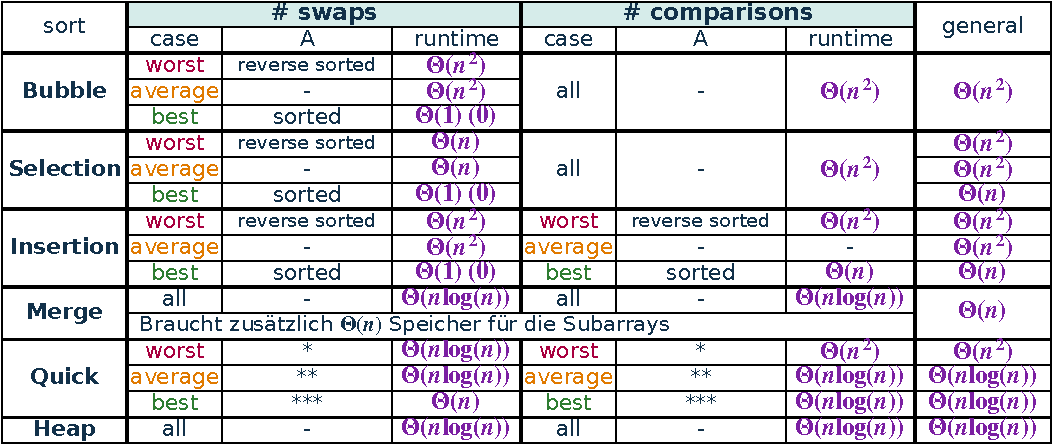
\includegraphics[width=\columnwidth]{Images/algorithm-sorting-complexity-swaps-comparisons.pdf}
\end{center}
\end{contentbox}

%=====================================================================================================================
\subsection{Quadratische Sortierverfahren}\label{sec:04-quadratische-sortierverfahren}
\subsubsection{Bubble Sort}\label{sec:04-bubble-sort}
\ZSFindex{Bubble Sort}
\begin{center}
    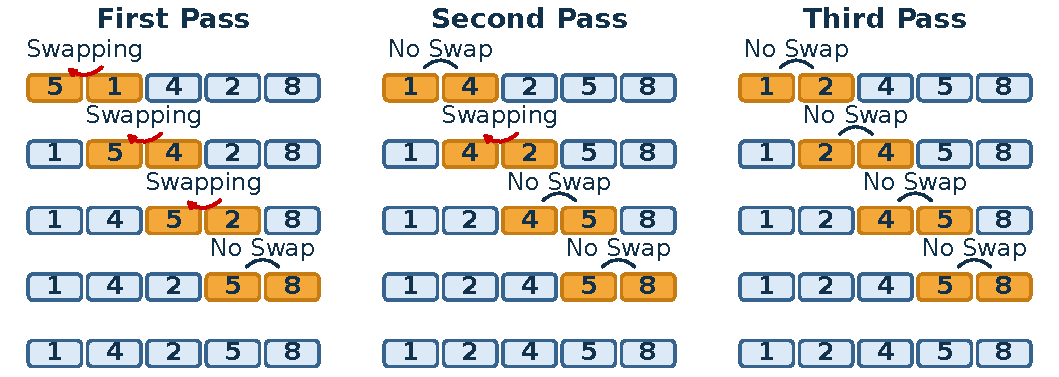
\includegraphics[width=\columnwidth]{Images/algorithm-bubble-sort-passes.pdf}
\end{center}

\begin{procedure}[Ablauf]
\ProcStep{Vergleichen \& Tauschen}{Vergleicht benachbarte Elemente und vertauscht sie bei falscher Reihenfolge.}
\ProcStep{Wiederholen}{Wiederholt dies, bis keine Vertauschungen mehr nötig sind.}
\end{procedure}
\begin{contentbox}
\begin{factlist}
\ZSFFact{Invariante}{\texttt{a[:-(i + 1)]} enthält die $i + 1$ grössten Elemente von \texttt{a} in sort. Reihe.}
\ZSFFact{Laufzeit}{$\Theta(n^2)$ im Durchschnitt und schlechtesten Fall.}
\end{factlist}
\end{contentbox}
\begin{codebox}[Bubble Sort (In-Place, mutiert Array)]
\begin{lstlisting}[style=CodeExpert]
def bubble_sort(a):
    n = len(a)
    # Grosse Schleife über alle Elemente
    for i in range(n):
        # Vergleicht bis zum unsortierten Rest
        for j in range(0, n-i-1):
            # Wenn linkes Element grösser...
            if a[j] > a[j+1]:
                # ...vertausche beide
                a[j], a[j+1] = a[j+1], a[j]
\end{lstlisting}
\end{codebox}

\subsubsection{Selection Sort}\label{sec:04-selection-sort}
\ZSFindex{Selection Sort}
\begin{center}
    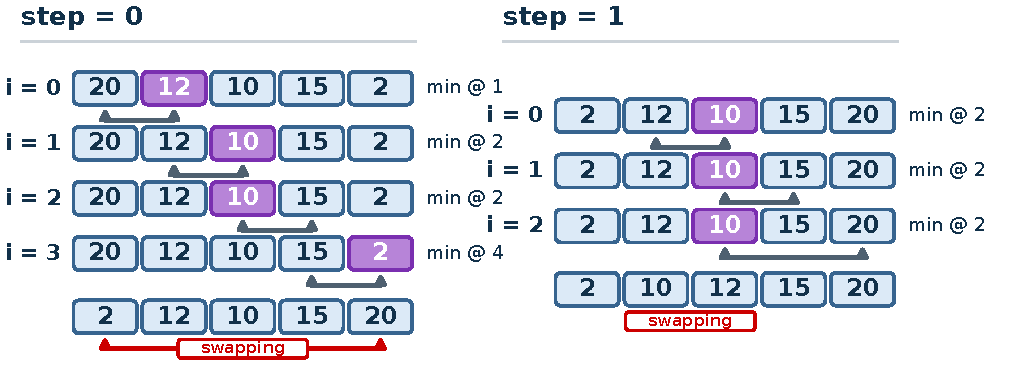
\includegraphics[width=\columnwidth]{Images/algorithm-selection-sort-passes.pdf}
\end{center}
\begin{procedure}[Ablauf]
\ProcStep{Minimum suchen}{Sucht in jedem Durchlauf das kleinste Element.}
\ProcStep{Tauschen}{Tauscht es mit dem aktuellen Element.}
\ProcStep{Wiederholen}{Wiederholt das für den restlichen unsortierten Bereich.}
\end{procedure}
\begin{contentbox}
\begin{factlist}
\ZSFFact{Invariante}{\texttt{a[:i + 1]} enthält die kleinsten \(i + 1\) Elemente von \texttt{a}, in sort. Reihe.}
\ZSFFact{Laufzeit}{$\Theta(n^2)$ in allen Fällen.}
\end{factlist}
\end{contentbox}
\begin{codebox}[Selection Sort (In-Place, mutiert Array)]
\begin{lstlisting}[style=CodeExpert]
def selection_sort(a):
    n = len(a)
    # Grosse Schleife über alle Positionen
    for i in range(n):
        # Nimm an, dass a[i] das Minimum ist
        min_idx = i
        # Suche im restlichen Feld...
        for j in range(i+1, n):
            # ...nach einem noch kleineren Element
            if a[j] < a[min_idx]:
                # Speichere neuen Index des Minimums
                min_idx = j
        # Tausche an sortierte Position
        a[i], a[min_idx] = a[min_idx], a[i]
\end{lstlisting}
\end{codebox}




\subsubsection{Insertion Sort}\label{sec:04-insertion-sort}
\ZSFindex{Insertion Sort}
\begin{center}
    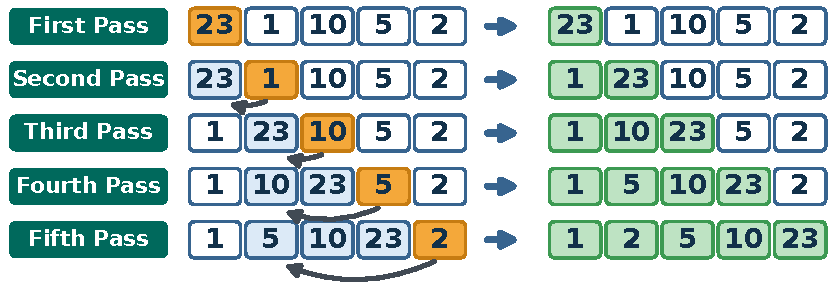
\includegraphics[width=\columnwidth]{Images/algorithm-insertion-sort-passes.pdf}
\end{center}
\begin{procedure}[Ablauf]
\ProcStep{Idee}{Sortiert ähnlich wie beim Kartenspiel.}
\ProcStep{Einfügen}{Jedes Element wird an die richtige Position im linken, bereits sortierten Teil eingefügt.}
\ProcStep{Verschieben}{Grössere Elemente werden nach rechts verschoben.}
\end{procedure}
\begin{contentbox}
\begin{factlist}
\ZSFFact{Invariante}{Die Elemente in \texttt{a[:i + 1]} sind sortiert und entsprechen den ersten $i$ Elementen des ursprüngl. Arrays.}
\ZSFFact{Laufzeit}{$\Theta(n)$ im besten Fall (wenn sortiert), $\Theta(n^2)$ im Worst-Case.}
\end{factlist}
\end{contentbox}
\begin{codebox}
\begin{lstlisting}[style=CodeExpert]
def insertion_sort(a):
    # Starte beim zweiten Element
    for i in range(1, len(a)):
        # Speichere aktuelles Element
        key = a[i]
        # Betrachte die Elemente links davon
        j = i - 1
        # Solange links grössere Elem. sind
        while j >= 0 and key < a[j]:
            # Verschiebe sie nach rechts
            a[j + 1] = a[j]
            # Gehe weiter nach links
            j -= 1
        # Füge das Element an Lücke ein
        a[j + 1] = key
\end{lstlisting}
\end{codebox}




\subsection{Divide-and-Conquer-Sortierung}\label{sec:04-divide-and-conquer-sortierung}
\ZSFindex{Divide and Conquer}
\subsubsection{Merge Sort}\label{sec:04-merge-sort}
\ZSFindex{Merge Sort}
\begin{center}
    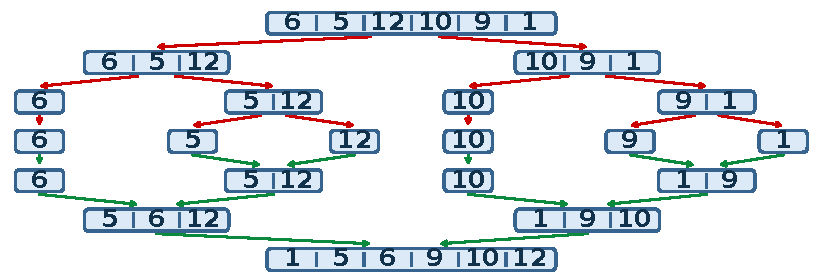
\includegraphics[width=\columnwidth]{Images/algorithm-merge-sort-split-merge-tree.pdf}
\end{center}
\begin{procedure}[Ablauf]
\ProcStep{Idee}{Rekursiver Divide-and-Conquer-Algorithmus.}
\ProcStep{Teilen}{Das Array wird in zwei Hälften geteilt.}
\ProcStep{Rekursiv sortieren}{Beide Hälften werden rekursiv sortiert.}
\ProcStep{Zusammenführen}{Die sortierten Hälften werden zusammengeführt (merge).}
\end{procedure}
\begin{contentbox}
\begin{factlist}
\ZSFFact{Invariante}{Das Resultat-Array \texttt{b[:i + 1]} enthält die $i + 1$ kleinsten Elemente von \texttt{a} in sortierter Reihenfolge.}
\ZSFFact{Laufzeit}{$\Theta(n \log n)$ in allen Fällen.}
\end{factlist}
\end{contentbox}
\begin{codebox}
\begin{lstlisting}[style=CodeExpert]
def merge_sort(a):
    # Wenn Array mehr als 1 Element hat
    if len(a) > 1:
        # Finde die Mitte
        mid = len(a) // 2
        # Teile das Array in zwei Hälften
        L, R = a[:mid], a[mid:]
        # Sortiere beide rekursiv
        merge_sort(L); merge_sort(R)
        i = j = k = 0
        # Beide Hälften zusammenfügen
        while i < len(L) and j < len(R):
            # Nimm das kleinere Element ...
            if L[i] < R[j]:
                # ...aus linker Hälfte
                a[k] = L[i]; i+=1
            else:
                # ...aus rechter Hälfte
                a[k] = R[j]; j+=1
            k+=1
        # Rest links anhängen
        while i < len(L):
            a[k] = L[i]; i+=1; k+=1
        # Rest rechts anhängen
        while j < len(R):
            a[k] = R[j]; j+=1; k+=1
\end{lstlisting}
\end{codebox}


\subsubsection{Quick Sort}\label{sec:04-quick-sort}
\ZSFindex{Quick Sort}
\begin{center}
    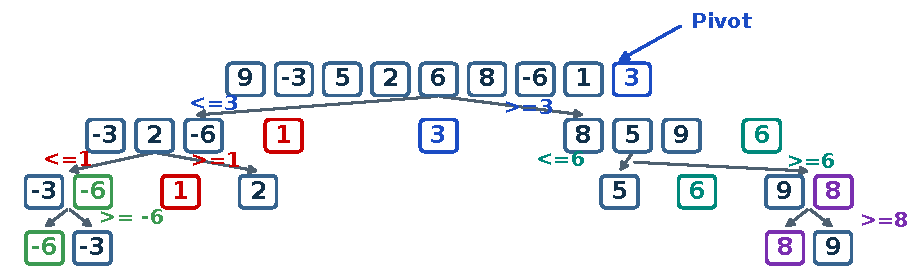
\includegraphics[width=\columnwidth]{Images/algorithm-quicksort-pivot-partition-tree.pdf}
\end{center}
\begin{procedure}[Ablauf]
\ProcStep{Idee}{Effizienter rekursiver Divide-and-Conquer-Algorithmus.}
\ProcStep{Pivot wählen}{Wählt ein \ZSFkeyword*{Pivot}-Element.}
\ProcStep{Partitionieren}{Teilt das Array in Elemente kleiner und grösser als das Pivot.}
\ProcStep{Rekursiv sortieren}{Sortiert beide Teilarrays rekursiv.}
\end{procedure}
\begin{contentbox}
\begin{factlist}
\ZSFFact{Invariante}{Das Pivotelement befindet sich an der richtigen Posit., Elem. links davon sind kleiner und rechts davon grösser als das Pivot.}
\ZSFFact{Laufzeit}{$\Theta(n \log n)$ durchschnittlich, $\Theta(n^2)$ im Worst-Case.}
\end{factlist}
\end{contentbox}
\begin{codebox}
\begin{lstlisting}[style=CodeExpert]
def quick_sort(a, low, high):
    # Wenn mehr als ein Element da ist
    if low < high:
        # Wähle ganz rechts als Pivot
        pivot = a[high]
        # Zeiger für kleineres Element
        i = low - 1
        # Gehe durch das Array
        for j in range(low, high):
            # Wenn Element kleiner/gleich Pivot
            if a[j] <= pivot:
                # Verschiebe Zeiger
                i += 1
                # Vertausche Elemente
                a[i], a[j] = a[j], a[i]
        # Setze Pivot in die Mitte
        a[i+1], a[high] = a[high], a[i+1]
        # Dies ist die fertige Pivot-Position
        pi = i + 1
        # Sortiere rekursiv links vom Pivot
        quick_sort(a, low, pi - 1)
        # Sortiere rekursiv rechts vom Pivot
        quick_sort(a, pi + 1, high)
\end{lstlisting}
\end{codebox}




\subsection{Heap-basierte Sortierung}\label{sec:04-heap-basierte-sortierung}
\subsubsection{Heap Sort}\label{sec:04-heap-sort}
\ZSFindex{Heap Sort}
\begin{center}
    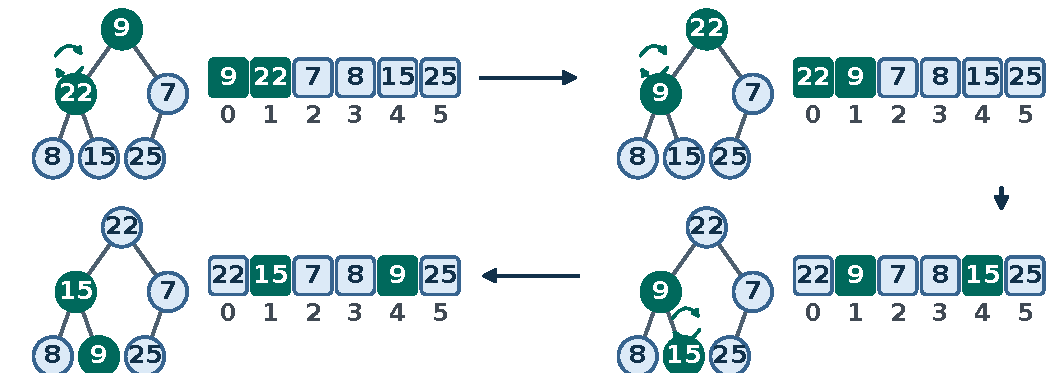
\includegraphics[width=\columnwidth]{Images/algorithm-heapsort-max-heap-extraction.pdf}
\end{center}
\begin{procedure}[Ablauf]
\ProcStep{Max-Heap aufbauen}{Erst wird ein Max-Heap aufgebaut. \ZSFref{sec:06-heaps}}
\ProcStep{Wurzel entnehmen}{Grösstes Element (Wurzel) wird entfernt und ans Ende gesetzt.}
\ProcStep{Heapify}{Der Heap wird danach angepasst (heapify).}
\end{procedure}
\begin{contentbox}
\begin{factlist}
\ZSFFact{Laufzeit}{$\Theta(n \log n)$ in allen Fällen.}
\end{factlist}
\end{contentbox}
\begin{codebox}[Heapify (Max-Heap)]
\begin{lstlisting}[style=CodeExpert]
def heapify(a, n, i):
    # Setze root als grösstes Element
    largest = i
    # Linkes und rechtes Kind
    l, r = 2 * i + 1, 2 * i + 2
    # Kind links grösser?
    if l < n and a[l] > a[largest]: largest = l
    # Kind rechts grösser?
    if r < n and a[r] > a[largest]: largest = r
    # Wenn Root nicht das Grösste ist...
    if largest != i:
        # ...vertausche beide
        a[i], a[largest] = a[largest], a[i]
        # Max-Heap-Eigenschaft wiederherst.
        heapify(a, n, largest)
\end{lstlisting}
\end{codebox}

\begin{codebox}[Heap Sort]
\begin{lstlisting}[style=CodeExpert]
def heap_sort(a):
    n = len(a)
    # Baue einen Max-Heap auf (bottom-up)
    for i in range(n//2 - 1, -1, -1):
        heapify(a, n, i)
    # Elemente einzeln entnehmen
    for i in range(n-1, 0, -1):
        # Aktuelle Wurzel ans Ende setzen
        a[i], a[0] = a[0], a[i]
        # Erneut Max-Heap aufbauen
        heapify(a, i, 0)
\end{lstlisting}
\end{codebox}




\subsection{Binäre Suche beim Einfügen}\label{sec:04-binaere-suche-beim-einfuegen}
\ZSFindex[binare-suche]{Binäre Suche}
\subsubsection{Binary Insertion Sort}\label{sec:04-binary-sort}
\begin{center}
    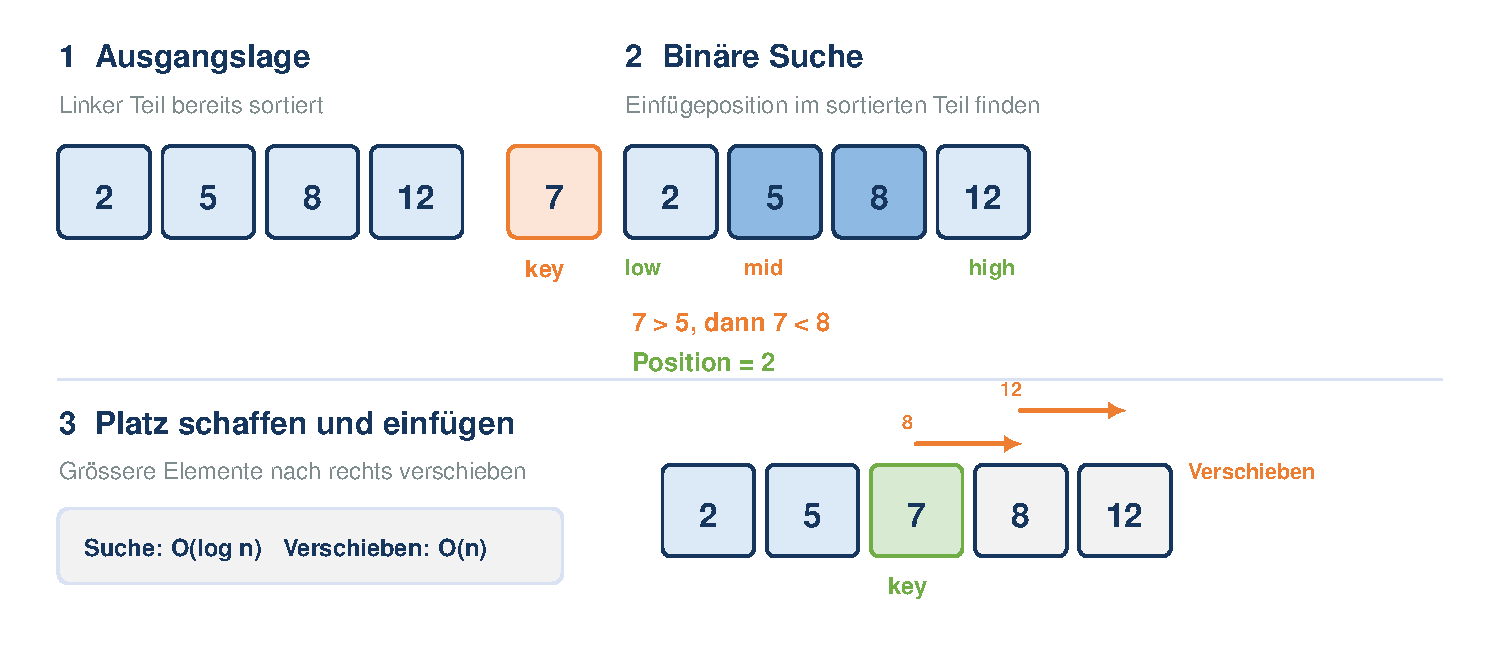
\includegraphics[width=\columnwidth]{Images/algorithm-binary-insertion-sort-search-shift-insert.pdf}
\end{center}
\begin{procedure}[Ablauf]
\ProcStep{Idee}{Eine Variante von Insertion Sort.}
\ProcStep{Binär suchen}{Findet die Einfügeposition per binärer Suche.}
\ProcStep{Verschieben}{Die Verschiebung der Elemente bleibt aber linear.}
\end{procedure}
\begin{contentbox}
\begin{factlist}
\ZSFFact{Laufzeit}{$\Theta(n^2)$ (Vergleiche: $\Theta(n \log n)$, Verschiebungen: $\Theta(n^2)$).}
\end{factlist}
\end{contentbox}
\begin{codebox}
\begin{lstlisting}[style=CodeExpert]
def binary_insertion_sort(a):
    # Starte beim zweiten Element
    for i in range(1, len(a)):
        key = a[i]  # Zu fügendes Element
        # --- 1. Binäre Suche nach Einfügeposition ---
        low, high = 0, i - 1
        while low <= high:
            mid = (low + high) // 2
            # Suche in linker Hälfte
            if key < a[mid]: high = mid - 1
            # Suche in rechter Hälfte
            else: low = mid + 1
        # --- 2. Elemente nach rechts verschieben ---
        for j in range(i, low, -1):
            a[j] = a[j - 1]  # Eins nach rechts
        a[low] = key         # Setze an gefundene Pos.
\end{lstlisting}
\end{codebox}
